% Title: Software Requirements Specification
% Project: BusMate
% Version: 3

\documentclass{BusMateSRS}
\usepackage{graphicx} 
\usepackage{caption, subcaption} 

\def\projectName{BusMate}
\def\projectShortDescription{Real-Time Microbus Transportation System}
\def\docVersion{Version 3}

\def\nameAndrew{Andrew Amin}
\def\nameKarim{Karim Muhammad}
\def\nameHamdy{Muhammad Hamdy}
\def\nameHossam{Muhammad Hossam}
\def\docAuthors{\nameAndrew \and \nameKarim \and \nameHamdy \and \nameHossam}

\def\pubDepartment{Department of Computer and Systems Engineering}
\def\pubFaculty{Faculty of Engineering}
\def\pubUniveristy{Helwan University}
\def\docPublishers{\pubDepartment, \pubFaculty, \pubUniveristy}


\begin{document}
\maketitle
\tableofcontents
\listoffigures
\listoftables

%-%-%-%-%-%-%-%-%-%-%-%-%-%-%-%-%-%-%-%-%-%-%-%-%-%-%-%-%-%-%-%-%-%-%-%-%-%-%-%
%-%-%-%-%-%-%-%-%-%-%-%-%-%-%-%-%-%-%-%-%-%-%-%-%-%-%-%-%-%-%-%-%-%-%-%-%-%-%-%
\chapter*{Revision History}
\begin{table}[ht!]
	\centering
	\begin{tabularx}{\textwidth}{|c|l|l|X|}
		\hline
		\textbf{Version} & \textbf{Date} & \textbf{Edited By} & \textbf{Description} \\
		\hline
		1                & Oct 18, 2023  & \nameAndrew        &
		Initial functional requirements and users definition                         \\
		\hline
		1                & Oct 21, 2023  & \nameKarim         &
		Initial interface and non-functional requirements                            \\
		\hline
		1                & Oct 22, 2023  & \nameHamdy         &
		Project purpose, scope and redefine users                                    \\
		\hline
		1                & Oct 23, 2023  & \nameHossam        &
		System architecture and block diagram                                        \\
		\hline
		2                & Nov 7, 2023   & \nameAndrew        &
		Rewrite functional requirements, purpose and scope                           \\
		\hline
		2                & Dec 2, 2023   & \nameHamdy         &
		Designed the database as an entity relationship diagram                      \\
		\hline
		2                & Dec 5, 2023   & \nameHossam        &
		Designed the use-case diagram                                                \\
		\hline
		2                & Dec 5, 2023   & \nameAndrew        &
		Designed the class diagram                                                   \\
		\hline
		2                & Dec 7, 2023   & \nameKarim         &
		Added various classes and revised whole document                             \\
		\hline
		3                & Dec 21, 2023   & \nameHamdy        &
		Added relational model diagram                                               \\
		\hline
		3                & Dec 26, 2023   & \nameKarim &
		Edited database and class diagrams \\
		\hline
		3                & Dec 26, 2023   & \nameHamdy        &
		Added sequence diagram \\
		\hline
	\end{tabularx}
	\caption{Revision History}
	\label{tab:revision-history}
\end{table}

%-%-%-%-%-%-%-%-%-%-%-%-%-%-%-%-%-%-%-%-%-%-%-%-%-%-%-%-%-%-%-%-%-%-%-%-%-%-%-%
%-%-%-%-%-%-%-%-%-%-%-%-%-%-%-%-%-%-%-%-%-%-%-%-%-%-%-%-%-%-%-%-%-%-%-%-%-%-%-%

\chapter{Introduction}
\section{Purpose}
The purpose of the Software Requirements Specification (SRS) is to provide
a detailed description of the Microbus Transportation Web Application.
It serves as a comprehensive document that outlines the functional and
non-functional requirements, constraints, and dependencies of the system.

The SRS acts as a reference for the development team, stakeholders, and anyone
involved in the project to understand the scope, objectives, and specifications
of the application.


\section{Scope}
\emph{\projectName}, The Microbus Transportation Web Application aims to
connect microbus drivers and passengers in real-time.
It addresses the challenge of passengers waiting for microbuses that
do not align with their needs, while drivers are unaware of potential passengers
along their routes.

The application seeks to improve the transportation experience by providing
a platform for efficient communication and coordination between drivers and
passengers.


\section{Definitions, Acronyms, and Abbreviations}
\begin{itemize}
	\item {\projectName}:
	      The name of project
	\item SRS:
	      Software Requirements Specification
	\item IEEE:
	      Institute of Electrical and Electronics Engineers
	\item Microbus:
	      A small public transportation vehicle that can accommodate
	      a limited number of passengers.
	\item Passenger:
	      An individual who intends to use the microbus transportation service.
	\item Driver:
	      An individual who operates a microbus and provides transportation
	      services to passengers.
	\item Web Application:
	      A software application that is accessed through a web browser and provides
	      functionality and services over the internet.
	\item Real-time: The ability to provide and receive information
	      instantaneously or with minimal delay.
\end{itemize}

\section{References}
\begin{itemize}
	\item IEEE Std 830-1998: IEEE Recommended Practice for Software Requirements
	      Specifications, \url{http://www.math.uaa.alaska.edu/~afkjm/cs401/IEEE830.pdf}.
\end{itemize}

%% TODO:
% \section{Overview}
% This subsection should
% a) Describe what the rest of the SRS contains;
% b) Explain how the SRS is organized.


%-%-%-%-%-%-%-%-%-%-%-%-%-%-%-%-%-%-%-%-%-%-%-%-%-%-%-%-%-%-%-%-%-%-%-%-%-%-%-%
\chapter{Overall Description}
\section{Product Perspective}
The Microbus Transportation Web Application will be a standalone system,
interacting with microbus drivers and passengers through a user-friendly
web interface. It will not rely on any external systems for its core
functionality, but may utilize geolocation services and payment gateways for
additional features.

\section{Product Features}
\begin{itemize}
	\item Real-time microbus tracking and availability display
	\item Passenger registration and profile management
	\item Driver registration and profile management
	\item Route selection and scheduling for drivers
	\item Passenger search and booking for available microbuses
	\item Notifications for drivers and passengers regarding trip updates
\end{itemize}

\section{User Classes and Characteristics}
The Microbus Transportation Web Application will have two primary user classes:
passengers and drivers. Passengers will include individuals who rely on
microbuses for transportation, while drivers will be microbus owners or
operators.
Both user classes are expected to have basic computer literacy and
access to the internet.
We prototyped a block diagram as in figure \ref{fig:system-block-diagram}.

\begin{figure}[ht!]
	\centering
	\includegraphics[width=\columnwidth]{drawings/system-block-diagram.drawio.png}
	\caption{System Block Diagram}
	\label{fig:system-block-diagram}
\end{figure}

\pagebreak

%-%-%-%-%-%-%-%-%-%-%-%-%-%-%-%-%-%-%-%-%-%-%-%-%-%-%-%-%-%-%-%-%-%-%-%-%-%-%-%
\chapter{Specific Requirements}
\section{External Interface Requirements}
\subsection{User Interfaces}
The web application will have a user-friendly interface with intuitive
navigation and clear instructions. It will support multiple devices and
provide accessibility features for users with disabilities.
We have prototyped some user interfaces as in figures
\ref{fig:ui-prototype1}, \ref{fig:ui-prototype2} and \ref{fig:ui-prototype3}.

\subsubsection{General UI}
\begin{itemize}
	\item Welcome or login page:
	      includes login form and short description
	\item Create account:
	      includes registration form as either a driver or a passenger
\end{itemize}

\subsubsection{Driver UI}
\begin{itemize}
	\item Driver homepage:
	      includes hello message and buttons to start a trip, bank-card settings,
	      account settings, and logout
	\item Start trip:
	      includes cancel button and list of routes to choose from, delete, edit,
	      or add a new route.
	\item Driving now:
	      includes end trip button, complete/available radio buttons and
	      a list of notifications of passengers'
	      ride requests with accept/reject buttons, and fee amount
\end{itemize}

\subsubsection{Passenger UI}
\begin{itemize}
	\item Passenger homepage:
	      includes hello message and buttons to ride, bank-card settings,
	      account settings, and logout
	\item Ride:
	      includes a map with available routes pins to be clicked and a list
\end{itemize}

\begin{figure}[ht!]
	\centering
	\begin{subfigure}[b]{0.3\textwidth}
		\centering
		\includegraphics[width=\textwidth]{images-ui/ui-out-1.jpg}
		\caption{Welcome Page}
		\label{fig:ui1}
	\end{subfigure}
	\hfill
	\begin{subfigure}[b]{0.3\textwidth}
		\centering
		\includegraphics[width=\textwidth]{images-ui/ui-out-2.jpg}
		\caption{Create Account}
		\label{fig:ui2}
	\end{subfigure}
	\hfill
	\begin{subfigure}[b]{0.3\textwidth}
		\centering
		\includegraphics[width=\textwidth]{images-ui/ui-out-5.jpg}
		\caption{Account Settings}
		\label{fig:ui5}
	\end{subfigure}
	\hfill
	\begin{subfigure}[b]{0.3\textwidth}
		\centering
		\includegraphics[width=\textwidth]{images-ui/ui-out-6.jpg}
		\caption{Bank Card Settings}
		\label{fig:ui6}
	\end{subfigure}
	\caption{UI Prototype (General)}
	\label{fig:ui-prototype1}
\end{figure}

\begin{figure}[ht!]
	\centering
	\begin{subfigure}[b]{0.3\textwidth}
		\centering
		\includegraphics[width=\textwidth]{images-ui/ui-out-3.jpg}
		\caption{Driver Homepage}
		\label{fig:ui3}
	\end{subfigure}
	\hfill
	\begin{subfigure}[b]{0.3\textwidth}
		\centering
		\includegraphics[width=\textwidth]{images-ui/ui-out-7.jpg}
		\caption{Start Trip}
		\label{fig:ui7}
	\end{subfigure}
	\hfill
	\begin{subfigure}[b]{0.3\textwidth}
		\centering
		\includegraphics[width=\textwidth]{images-ui/ui-out-8.jpg}
		\caption{Driving Now}
		\label{fig:ui8}
	\end{subfigure}
	\hfill
	\begin{subfigure}[b]{0.3\textwidth}
		\centering
		\includegraphics[width=\textwidth]{images-ui/ui-out-9.jpg}
		\caption{Driving Now (Accept Example)}
		\label{fig:ui9}
	\end{subfigure}
	\caption{UI Prototype (Driver)}
	\label{fig:ui-prototype2}
\end{figure}

\begin{figure}[ht!]
	\centering
	\begin{subfigure}[b]{0.3\textwidth}
		\centering
		\includegraphics[width=\textwidth]{images-ui/ui-out-4.jpg}
		\caption{Passenger Homepage}
		\label{fig:ui4}
	\end{subfigure}
	\caption{UI Prototype (Passenger)}
	\label{fig:ui-prototype3}
\end{figure}

\subsection{Hardware Interfaces}
The application will run on standard hardware configurations,
including desktops, laptops, and mobile devices.
It will utilize GPS capabilities for real-time tracking.

\subsection{Software Interfaces}
The application will integrate with geolocation services for accurate tracking
and mapping. It will also integrate with payment gateways for secure online
transactions.

\section{Functional Requirements}
\subsection{Passenger Functionality}
\begin{enumerate}
	\item Register as a passenger by providing necessary details
	\item Search for available microbuses based on location and timing preferences
	\item View microbus details, including driver information and capacity
	\item Book a seat on a selected microbus
	\item Receive notifications regarding trip updates
\end{enumerate}

\subsection{Driver Functionality}
\begin{enumerate}
	\item Register as a driver by providing necessary details
	\item Create and manage routes, specifying pickup and drop-off points
	\item Set availability and capacity for each microbus
	\item Receive booking requests from passengers
	\item Confirm or reject booking requests
	\item Receive notifications regarding trip updates
\end{enumerate}

\subsection{Web Server Functionality}
\begin{enumerate}
	\item Send notifications to passengers
	\item Send notifications to drivers
\end{enumerate}

The previous functions are viewed as a use-case diagram in
figure \ref{fig:usecase-diagram} and sequence diagram in figure~\ref{fig:sequence-diagram}.

\begin{figure}[ht!]
	\begin{center}
		\includegraphics[width=\columnwidth]{drawings/usecase-diagram.drawio.png}
	\end{center}
	\caption{Use-case Diagram}
	\label{fig:usecase-diagram}
\end{figure}


\pagebreak

\begin{figure}[ht!]
	\begin{center}
		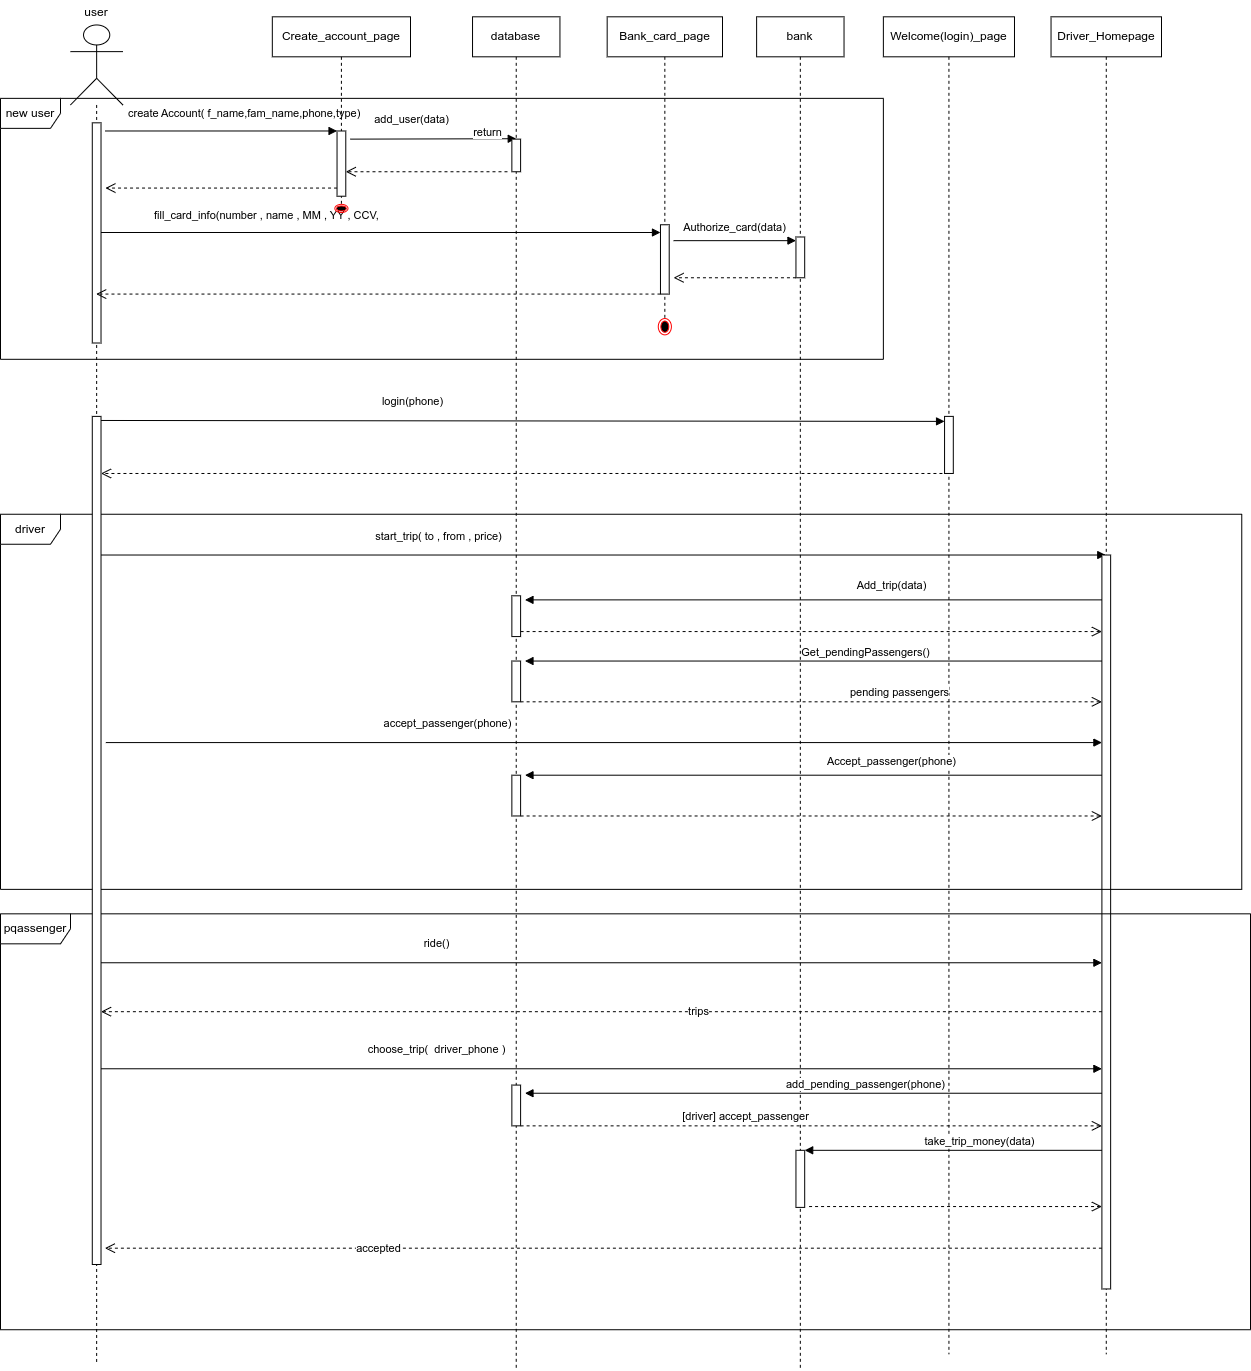
\includegraphics[width=\columnwidth]{drawings/sequence_diagram.drawio.png}
	\end{center}
	\caption{Sequence Diagram}
	\label{fig:sequence-diagram}
\end{figure}


\pagebreak


\section{Non-functional Requirements}
\subsection{Performance Requirements}
\begin{itemize}
	\item The application should be able to handle a large number of simultaneous
	      users without significant performance degradation.
	\item Real-time tracking and updates should have minimal delay,
	      providing accurate information to both drivers and passengers.
	\item The application should be responsive and provide a seamless user
	      experience, with quick loading times and minimal downtime for maintenance.
\end{itemize}


%-%-%-%-%-%-%-%-%-%-%-%-%-%-%-%-%-%-%-%-%-%-%-%-%-%-%-%-%-%-%-%-%-%-%-%-%-%-%-%
\section{System Design}

\subsection{Database Design}

The initial prototyping of the database is included in figures
\ref{fig:entity-relationship-diagram} and 
\ref{fig:relational-model}.

\begin{figure}[ht!]
	\begin{center}
		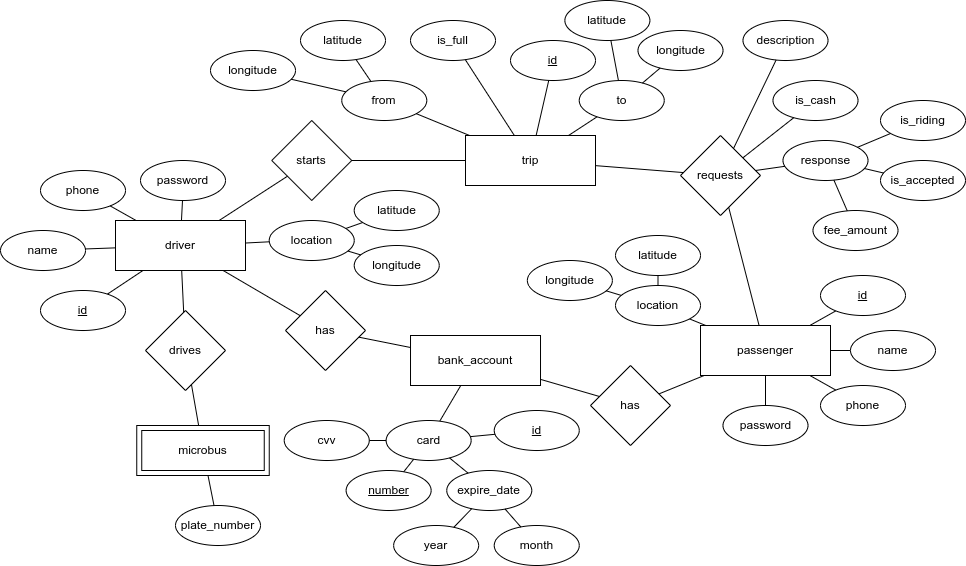
\includegraphics[width=\columnwidth]{drawings/entity-relationship-diagram.drawio.png}
	\end{center}
	\caption{Entity Relationship Diagram}
	\label{fig:entity-relationship-diagram}
\end{figure}

\begin{figure}[ht!]
	\begin{center}
		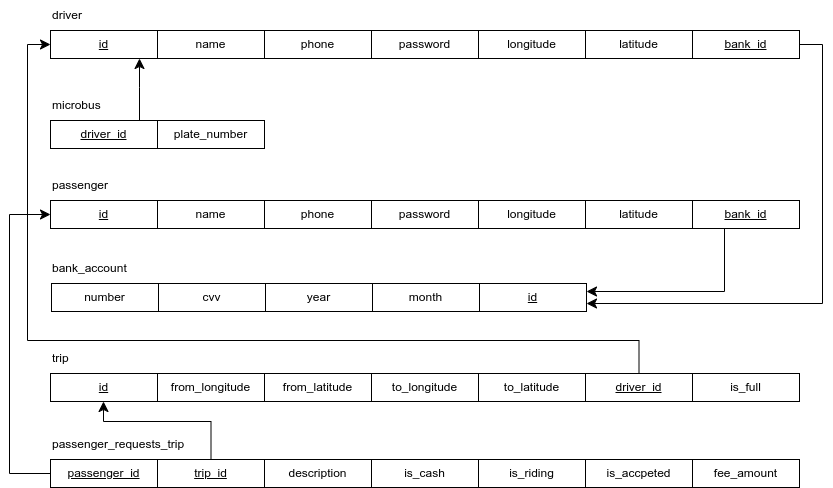
\includegraphics[width=\columnwidth]{drawings/relational-model.drawio.png}
	\end{center}
	\caption{Relational Model Diagram}
	\label{fig:relational-model}
\end{figure}

\pagebreak

\subsection{Class Diagram}
The initial class diagram of the application is included in figure
\ref{fig:class-diagram}.

\begin{figure}[ht!]
	\begin{center}
		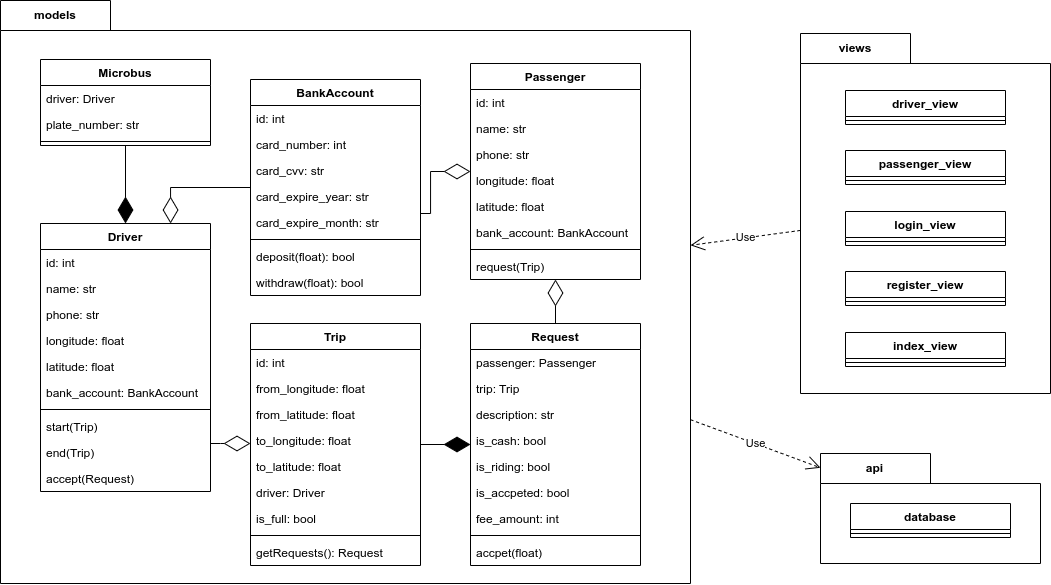
\includegraphics[width=\columnwidth]{drawings/class-diagram.drawio.png}
	\end{center}
	\caption{Class Diagram}
	\label{fig:class-diagram}
\end{figure}

\pagebreak


%-%-%-%-%-%-%-%-%-%-%-%-%-%-%-%-%-%-%-%-%-%-%-%-%-%-%-%-%-%-%-%-%-%-%-%-%-%-%-%
\section{Organizational Requirements}
The organizational requirements for the our project are as follows:

\begin{enumerate}
	\item Experienced developers familiar with Python, Flask, SQL,
	      GPS API, and Google Maps API.
	\item Clear roles and responsibilities assigned to team members.
	\item Regular communication and collaboration within the team.
	\item Adequate resources provided for development and testing.
	\item Well-defined project timeline with milestones and deliverables.
	\item Stakeholder meetings to gather feedback and incorporate requirements.
	\item Documentation maintained throughout the development process.
\end{enumerate}


%-%-%-%-%-%-%-%-%-%-%-%-%-%-%-%-%-%-%-%-%-%-%-%-%-%-%-%-%-%-%-%-%-%-%-%-%-%-%-%
%-%-%-%-%-%-%-%-%-%-%-%-%-%-%-%-%-%-%-%-%-%-%-%-%-%-%-%-%-%-%-%-%-%-%-%-%-%-%-%
\end{document}

